\section{Linear Quadratic Regulator} \label{sec:lqr}
\fxnote{Make Matrix Appendix with numbers}
\fxnote{Refference to matrix appendix where appropriate in this section.}
%
It is desired to design a state feedback using a linear quadratic regulator (LQR). 

\subsection{State Space Model}
The linearized model derived in \autoref{sec:linearizationModel}, consisting of \autoref{eq:x_pos_model_lin} to \ref{eq:psi_model_lin}, needs to be represented in state space form in order to design a state space controller. In order to do that, the 3 degree of freedom model used for the control of the vessel is represented as
\begin{flalign}
    \vec{\dot{x}}(t) &= \vec{A} \vec{x}(t) + \vec{B} \vec{u}(t)
    \label{xDotLinear} \\
    \vec{y}(t) &= \vec{C} \vec{x}(t) + \vec{D} \vec{u}(t)
    \label{yLinear} 
\end{flalign}
\begin{where}
    \va{\vec{x}}{is the state vector}{}
    \va{\vec{u}}{is the input vector}{}
    \va{\vec{y}}{is the output vector}{}
    \va{\vec{A}}{is the state matrix}{}
    \va{\vec{B}}{is the input matrix}{}
    \va{\vec{C}}{is the output matrix}{}
    \va{\vec{D}}{is the feed-forward matrix}{}
\end{where}

The state vector is constituted by the angle and velocity in yaw as well as the velocity in x in the body frame. The outputs of the system are yaw angle and velocity in x in the body frame. The input to the system is composed of the two forces applied in the body frame.
%It is important to notice that the position of the vessel in the body reference frame represents the  integration of the velocity along the body frame directions.
%This can also be seen as the position of the vessel with respect to a frame whose origin coincides with that of the NED frame and whose orientation coincides with that of the body frame \cite[p. 173]{TFossen}. 

\begin{minipage}{0.32\linewidth}
    \begin{flalign}
        \vec{x(t)} = 
        \begin{bmatrix}
            \psi\\
            \dot{\psi}\\
            \dot{x}_{b} \\
        \end{bmatrix} \nonumber
        \label{xVector}
    \end{flalign}  
\end{minipage}\hfill
%\hspace{0.03\linewidth}
\begin{minipage}{0.32\linewidth}
    \begin{flalign}
        \vec{y(t)} = 
        \begin{bmatrix}
            \phi \\
            \dot{x}_{b} \\
        \end{bmatrix} \nonumber
        \label{yVector}
    \end{flalign}
\end{minipage}\hfill
%\hspace{0.03\linewidth}
\begin{minipage}{0.32\linewidth}
    \begin{flalign}
        \vec{u(t)}= 
        \begin{bmatrix}
            F_1 \\
            F_2 
        \end{bmatrix}
        \label{uVector}
    \end{flalign} \nonumber
\end{minipage}\hfill

The resulting $\vec{A}$, $\vec{B}$, $\vec{C}$ and $\vec{D}$ matrices are
\begin{flalign}
    \vec{A} &=
    \begin{bmatrix}
        \ 0 & 1                   & 0                \ \ \ \\ 
        \ 0 & -\frac{d_\psi}{I_z} & 0                \ \ \ \\ 
        \ 0 & 0                   & -\frac{d_x}{m_x} \ \ \     
    \end{bmatrix}\rule{30px}{0px}
    \vec{B} = 
    \begin{bmatrix}
        \ 0               & 0                \ \ \ \\
        \ \frac{l_1}{I_z} & -\frac{l_2}{I_z} \ \ \ \\   
        \ \frac{1}{m_x}   & \frac{1}{m_x}    \ \ \
    \end{bmatrix}\rule{30px}{0px}
    \vec{C} =   
    \begin{bmatrix}
        \ 1 & 0 & 0  \ \ \ \\ 
        \ 0 & 0 & 1  \ \ \    
    \end{bmatrix}
    \label{eqStateSpaceABC}
\end{flalign}
and the $\vec{D}$ matrix is zero.

\subsection{Controller Design}
As the controller eventually must be implemented the design is carried out in the discrete domain. To do so, it is necessary to discretize the system. A discrete state space model can be expressed as,
%
\begin{flalign}
  \vec{x}(k+1) &= \vec{A_z} \vec{x}(k) + \vec{B_z} \vec{u}(k)
  \label{xDotLinearDiscrete} \\
  \vec{y}(k)   &= \vec{C_z} \vec{x}(k) + \vec{D_z} \vec{u}(k) \ \ ,
  \label{yLinearDiscrete} 
\end{flalign}
%
where the z subindexes indicate the matrices being in the discrete domain and k is the sample index. The model is discretized using zero order hold. In \autoref{fig:discreteSSBlock} the discrete system is shown in a block diagram. The feed forward matrix is excluded as it is not present in this system.
%
\begin{figure}[H]
  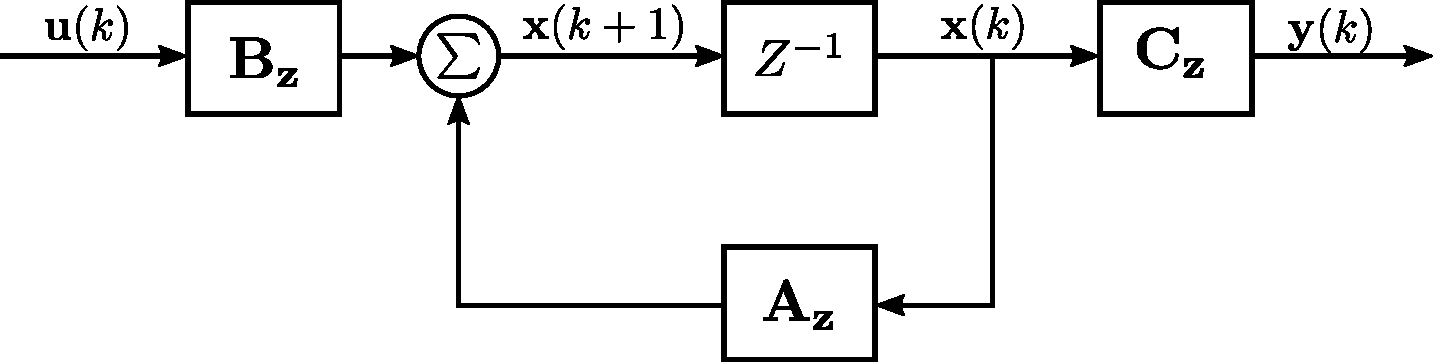
\includegraphics[width=0.6\textwidth]{figures/discreteSystemBlockDiagram}
  \caption{Block diagram of the discrete system without feed forward.}
  \label{fig:discreteSSBlock}
\end{figure}
%
In order to track a reference and handle input disturbances, it is chosen to also include an integral controller in the design. The final control structure is seen in \autoref{fig:blockConrolDesignLQR}.
%
\begin{figure}[H]
  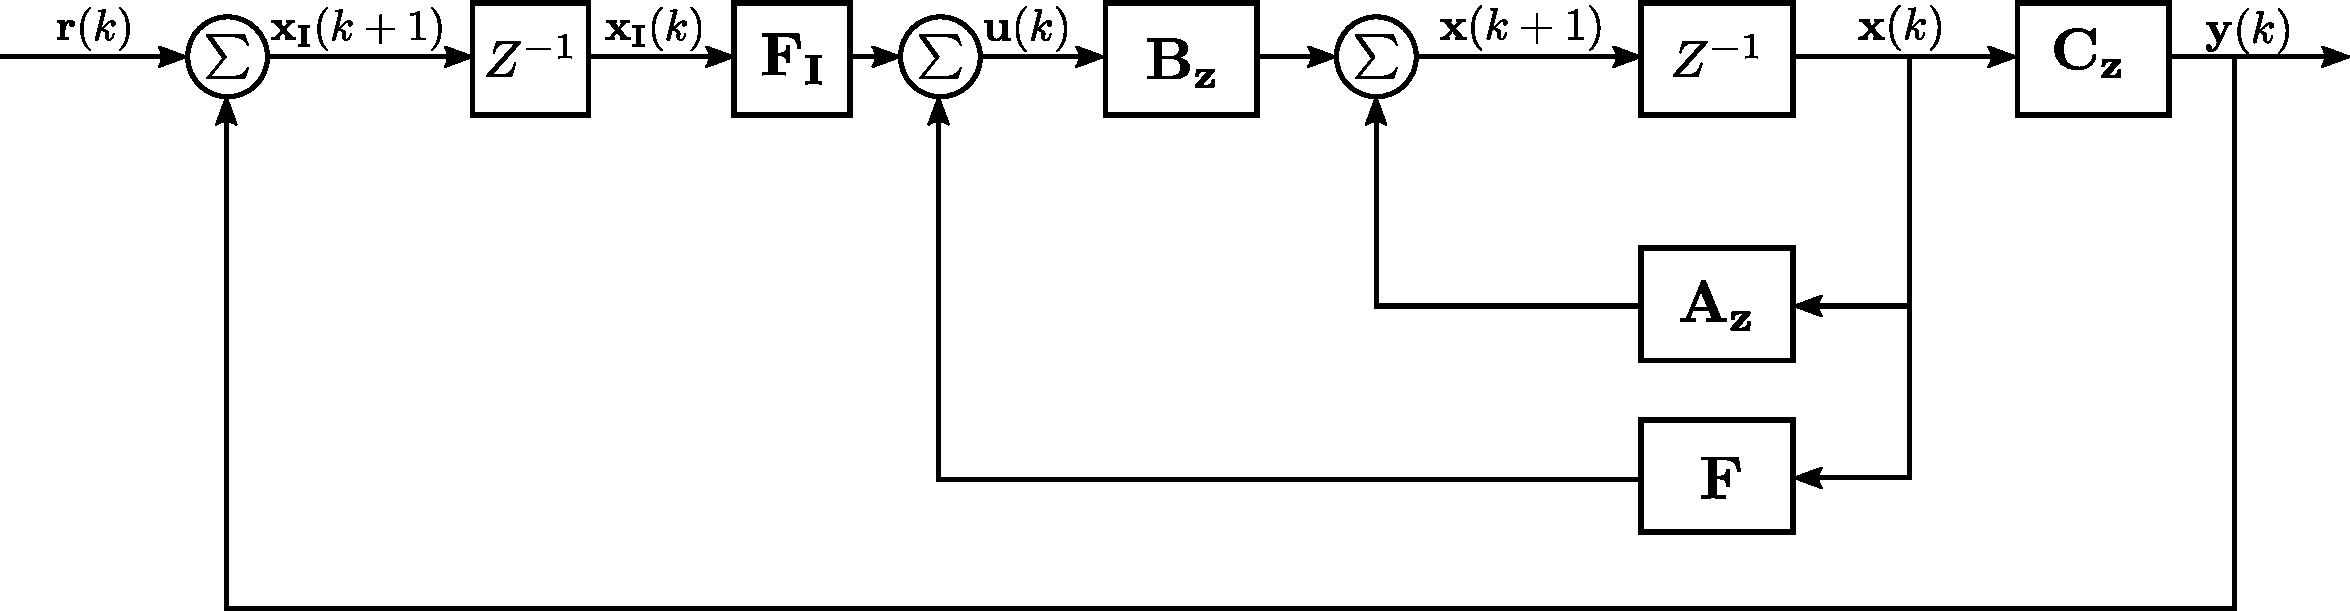
\includegraphics[width=0.9\textwidth]{figures/integralControlBlockDiagram}
  \caption{Block diagram of the control structure in the discrete domain.}
  \label{fig:blockConrolDesignLQR}
\end{figure}
%
To design this feedback system, it is convenient to express it on the following form:
\begin{flalign}
  \vec{x_e}(k+1) &= \vec{A_e} \vec{x}(k) + \vec{B_e} \vec{u}(k) + \vec{r}(k)
  \label{eq:xDotLinearDiscrete} \\
  \vec{y}(k)     &= \vec{C_e} \vec{x}(k)  \ \ .
  \label{eq:yLinearDiscrete} 
\end{flalign}
%
To describe the control design in this form, the $\vec{A_e}$, $\vec{B_e}$ and $\vec{C_e}$ matrices must be constructed. From \autoref{fig:blockConrolDesignLQR}, following relation is found:
%
\begin{flalign}
  \vec{x_I}(k+1) &= \vec{x_I}(k) + \vec{y}(k) + \vec{r}(k)    \nonumber \\
  \vec{x_I}(k+1) &= \vec{x_I}(k) - C_z \vec{x}(k) + \vec{r}(k)  \ \ .
  \label{eq:xIDiscrete}
\end{flalign}
%
This leads to the discrete state space model extended with the integral states expressed as
%
\begin{flalign}
  \begin{bmatrix}
    \vec{x}(k+1)  \\
    \vec{x_I}(k+1)
  \end{bmatrix}
  =
  \begin{bmatrix}
    \vec{A}_{\vec{z}_{3x3}} & \vec{O}_{_{3x2}} \\
   -\vec{C}_{\vec{z}_{2x3}} & \vec{I}_{_{2x2}} \\
  \end{bmatrix}
  \begin{bmatrix}
    \vec{x}(k)    \\
    \vec{x_I}(k)
  \end{bmatrix}
  +
  \begin{bmatrix}
    \vec{B}_{\vec{z}_{3x2}} \\
    \vec{O}_{2x2}
  \end{bmatrix}
  \vec{u}(k)
  +
  \begin{bmatrix}
    \vec{O}_{3x2} \\
    \vec{I}_{2x2}
  \end{bmatrix}
  \vec{r}(k)
  \label{eq:discreteSSWithIntegralX}
\end{flalign}  
%
\begin{flalign}
  \vec{y}(k)
  =
  \begin{bmatrix}
    \vec{C}_{\vec{z}_{2x3}} &  \vec{O}_{2x2}
  \end{bmatrix}
  \begin{bmatrix}
    \vec{x}(k)    \\
    \vec{x_I}(k)
  \end{bmatrix}  \ \ ,
  \label{eq:discreteSSWithIntegralY}
\end{flalign}  
%
which cooresponds to \autoref{eq:xDotLinearDiscrete} and \ref{eq:yLinearDiscrete}.

A discrete time infinite horizon LQR is used in the design of the feedback, $\vec{F_e} = [\ \vec{F} \ \ \vec{F}_\mathrm{I} ]\ $, which works by minimizing the cost function,
%
\begin{flalign}
  J = \sum_{k=0}^\infty \vec{x}_k^\mathrm{T}\vec{Q}\vec{x}_k + \vec{u}_k^\mathrm{T}\vec{R}\vec{u}_k  \ \ .
\end{flalign}
\begin{where}
	\va{\vec{Q}}{is the symmetric positive semidefinite state cost matrix}{}
  \va{\vec{R}}{is the symmetric positive definite input cost matrix}{}
\end{where}

The Q matrix contains the penalties for the state, such that a higher cost is generated for more critical states, thus driving these states faster to zero. The R matrix contains the penalties for the input. This helps to ensure that the actuators never enters saturation.\\
It is necessary for all states to be stable and controllable. Otherwise the the performance index, $J$, will become infinite \cite[p. 125]{DSNaidu}.\\
The controllability is determined by
%
\begin{flalign}
  \vec{{\mathcal C}}
  = 
  \begin{bmatrix}
    \vec{B}_\mathrm{e} & \vec{A}_\mathrm{e}\vec{B}_\mathrm{e} & \vec{A}_\mathrm{e}^\textbf{2} \vec{B}_\mathrm{e} & \vec{A}^\textbf{3}_\mathrm{e} \vec{B}_\mathrm{e} & \vec{A}^\textbf{4}_\mathrm{e} \vec{B}_\mathrm{e}
  \end{bmatrix}  \ \ ,
  \label{eq:integralControllability}
\end{flalign}
%
of which the rank is 5, that is, the controllability matrix, $\vec{{\mathcal C}}$, has full rank, thus the system is controllable \cite[p. 169]{CTChen}.\\
The eigenvalues of $\vec{A}_\mathrm{e}$ are all on or within the unit-circle in the z-plane, thus, no states are unstable and the LQR design is feasible.

Bryson's rule is used as an initial design method to determine sensible values for the state and input penalties in the Q and R matrices.
%
\begin{flalign} 
  Q_{ii} &= \frac{1}{x_{i_\mathrm{max}}\text{}^2} \rule{30px}{0px} R_{ii} = \frac{1}{u_{i_\mathrm{max}} \text{}^2}
  \label{eq:QRBryson}
\end{flalign}
\begin{where}
  \va{x_{i_\mathrm{max}}}{are the maximum acceptable state values}{}
  \va{u_{i_\mathrm{max}}}{are the maximum acceptable input values}{}
\end{where}

The requirements stated in \autoref{sec:requirements} must be taken into account when determining the values of $x_{i_\mathrm{max}}$ and $u_{i_\mathrm{max}}$.
\fxnote{Include arguments and numbers for final choice of Q and R.}

From this the state feedback is calculated by \cite[p. 42]{JLNy},
%
\begin{flalign}
  \vec{F}_\mathrm{e} &= -(\vec{B}_\mathrm{e}^\mathrm{T} \vec{P}\vec{B}_\mathrm{e} + \vec{R})^{-1}  \vec{B}_\mathrm{e}^\mathrm{T} \vec{P}\vec{A}_\mathrm{e} \ \ ,
  \label{eq:QRFeedback}
\end{flalign}
%
where $\vec{P}$ can be found as the solution of the infinite horizon algebraic discrete-time Riccati equation \cite[p. 42]{JLNy},
%
\begin{flalign}
\vec{P} &= \vec{A}_\mathrm{e}^\mathrm{T} \vec{P} \vec{A}_\mathrm{e} + \vec{Q} - \vec{A}_\mathrm{e}^\mathrm{T} \vec{P} \vec{B}_\mathrm{e} (\vec{B}_\mathrm{e}^\mathrm{T} \vec{P} \vec{B}_\mathrm{e} + \vec{R})^{-1} \vec{B}_\mathrm{e}^\mathrm{T} \vec{P} \vec{A}_\mathrm{e} \ \ .
\label{eq:discreteInfRiccati}
\end{flalign}
%
Once $\vec{F}_\mathrm{e}$ is obtained, it is split into the two feedback matrices, $\vec{F}_\mathrm{e} = [\ \vec{F} \ \ \vec{F}_\mathrm{I}\ ]$, and implemented, following the control structure provided in \autoref{fig:blockConrolDesignLQR}.










